

\begin{mydef}
	Un angle est défini par \kw{deux demi-droites de même origine}. Les demis droites sont les \kw{cotés} de l'angle et leur origine est son \kw{sommet}.
\end{mydef}

\begin{myex}
	\begin{multicols}{2}
		Cet angle est défini par les demi-droites $[BA)$ et $[BC)$. $[BA)$ et $[BC)$ sont ses cotés et $B$ est son sommet.
		On le note $\widehat{ABC}$ (le sommet de l'angle est toujours au milieu).
		
		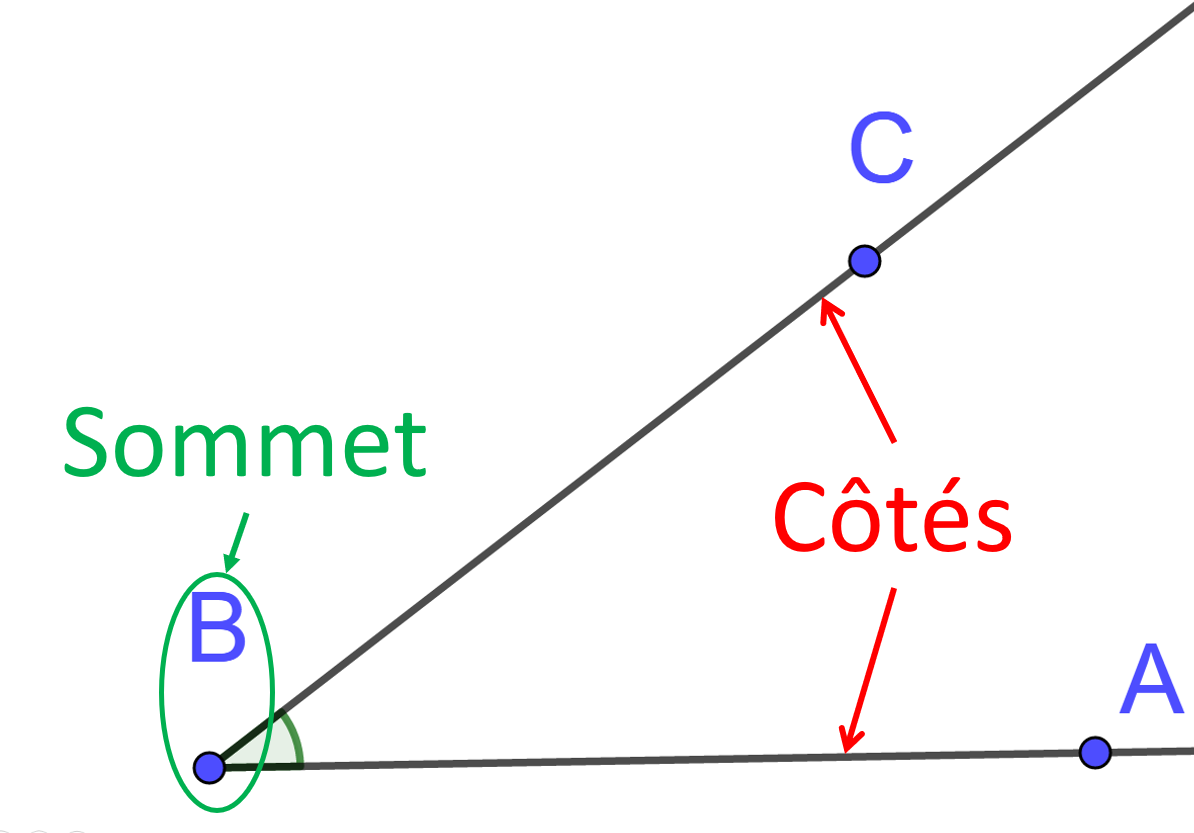
\includegraphics[scale=0.2]{ex1_1}
	\end{multicols}
\end{myex}